%%%%%%%% ICML 2021 EXAMPLE LATEX SUBMISSION FILE %%%%%%%%%%%%%%%%%

\documentclass{article}

% Recommended, but optional, packages for figures and better typesetting:
\usepackage{microtype}
\usepackage{graphicx}
\usepackage{subfigure}
\usepackage{booktabs} % for professional tables

% hyperref makes hyperlinks in the resulting PDF.
% If your build breaks (sometimes temporarily if a hyperlink spans a page)
% please comment out the following usepackage line and replace
% \usepackage{icml2021} with \usepackage[nohyperref]{icml2021} above.
\usepackage{hyperref}

% Attempt to make hyperref and algorithmic work together better:
\newcommand{\theHalgorithm}{\arabic{algorithm}}

% Use the following line for the initial blind version submitted for review:
\usepackage{icml2021}

% If accepted, instead use the following line for the camera-ready submission:
%\usepackage[accepted]{icml2021}

% The \icmltitle you define below is probably too long as a header.
% Therefore, a short form for the running title is supplied here:
\icmltitlerunning{Nonparametric tensor completion}
\usepackage{mathrsfs}
\usepackage{wrapfig}
\usepackage{multirow}
\usepackage{graphicx}
%\usepackage[utf8]{inputenc} % allow utf-8 input
%\usepackage[T1]{fontenc}    % use 8-bit T1 fonts
\usepackage{hyperref}       % hyperlinks
\usepackage{url}            % simple URL typesetting
%\usepackage{booktabs}       % professional-quality tables
\usepackage{amsmath,amssymb}
\usepackage{amsthm}    % blackboard math symbols
%\usepackage{nicefrac}       % compact symbols for 1/2, etc.
%\usepackage{microtype}      % microtypography
\usepackage{bm}
%\usepackage{subfig}
%\usepackage[english]{babel}
%\usepackage{algorithm}
%\usepackage{appendix}
\usepackage{mathtools}
\mathtoolsset{showonlyrefs}
\usepackage{enumitem}
\theoremstyle{plain}
\newtheorem{thm}{Theorem}[section]
\newtheorem{lem}{Lemma}
\newtheorem{prop}{Proposition}
\newtheorem{pro}{Property}


\theoremstyle{definition}
\newtheorem{defn}{Definition}
\newtheorem{assumption}{Assumption}
\newtheorem{cor}{Corollary}
\newtheorem{example}{Example}
\newtheorem{rmk}{Remark}

\usepackage{dsfont}
%\usepackage{algpseudocode,algorithm}
%\algnewcommand\algorithmicinput{\textbf{Input:}}
%\algnewcommand\algorithmicoutput{\textbf{Output:}}
%\algnewcommand\INPUT{\item[\algorithmicinput]}
%\algnewcommand\OUTPUT{\item[\algorithmicoutput]}
%\DeclareMathOperator*{\minimize}{minimize}

\usepackage{xr}



\newcommand*{\KeepStyleUnderBrace}[1]{%f
  \mathop{%
    \mathchoice
    {\underbrace{\displaystyle#1}}%
    {\underbrace{\textstyle#1}}%
    {\underbrace{\scriptstyle#1}}%
    {\underbrace{\scriptscriptstyle#1}}%
  }\limits
}
\usepackage{makecell}
\input macros.tex

\usepackage{amssymb}
\usepackage{pifont}
\newcommand{\cmark}{\ding{51}}%
\newcommand{\xmark}{\ding{55}}%
\def\sign{\textup{sgn}}
\def\srank{\textup{srank}}
\def\rank{\textup{rank}}
\def\caliP{\mathscr{P}_{\textup{sgn}}}
\def\risk{\textup{Risk}}

\begin{document}

\twocolumn[
\icmltitle{Beyond the Signs: Nonparametric Tensor Completion via Sign Series}

\icmlsetsymbol{equal}{*}

\begin{icmlauthorlist}
\icmlauthor{Chanwoo Lee}{wisc}
\icmlauthor{Miaoyan Wang}{wisc}
\end{icmlauthorlist}

\icmlaffiliation{wisc}{Department of Statistics, University of Wisconsin -- Madison}


\icmlcorrespondingauthor{Miaoyan Wang}{miaoyan.wang@wisc.edu}


% You may provide any keywords that you
% find helpful for describing your paper; these are used to populate
% the "keywords" metadata in the PDF but will not be shown in the document
\icmlkeywords{Higher-order tensors, completion, sliced inverse regression, probability estimation}

\vskip 0.3in
]

% this must go after the closing bracket ] following \twocolumn[ ...

% This command actually creates the footnote in the first column
% listing the affiliations and the copyright notice.
% The command takes one argument, which is text to display at the start of the footnote.
% The \icmlEqualContribution command is standard text for equal contribution.
% Remove it (just {}) if you do not need this facility.

\printAffiliationsAndNotice{}  % leave blank if no need to mention equal contribution


\begin{abstract}
We consider the problem of tensor estimation from noisy observations with possibly missing entries. A nonparametric approach to tensor completion is developed based on a new model which we coin as ``sign representable tensors.'' The model represents a real-valued signal tensor using a series of sign tensors with low sign ranks. Unlike earlier methods, the sign series representation enables effective analysis of high-rank signals, and also encompasses many existing low-rank tensor models---including CP models, Tucker models, single index models, certain hypergraphon models---as special cases. We show that the sign tensor series are theoretically characterized, and computationally estimable, by classification tasks with carefully-specified weights. The excess risk rate, estimation error bound, and sample complexity are established. The results uncover the joint contribution of statistical bias-variance errors and discretization errors. Numerical results demonstrate the robustness of our proposal over previous tensor methods.
\end{abstract}

\section{Introduction}\label{Intro}

\section{Preliminaries}
%Let $\Theta\in\mathbb{R}^{d_1\times \cdots \times d_K}$ denote a real-valued tensor. 
We use $\sign(\cdot)\colon \mathbb{R}\to\{-1,1\}$ to denote the sign function, where $\sign(y)=1$ if $y\geq 0$ and $-1$ otherwise. We allow univariate functions, such as $\sign(\cdot)$ or general $f\colon \mathbb{R}\to\mathbb{R}$, to be applied to tensors in an element-wise manner. We use the shorthand $[n]$ to denote the $n$-set $\{1,\ldots,n\}$ for $n\in\mathbb{N}_{+}$. We use $\otimes$ to denote the outer product of vectors, $\vnormSize{}{\mx}$ to denote the vector $2$-norm, and $\mathbb{S}^{d-1}=\{\mx\in\mathbb{R}\colon \vnormSize{}{\mx}=1\}$ to denote the $(d-1)$-dimensional unit sphere.

We use $\tY\in\mathbb{R}^{d_1\times \cdots \times d_K}$ to denote an order-$K$ $(d_1,\ldots,d_k)$-dimensional tensor, and use $\tY(\omega)\in\mathbb{R}$ to denote the tensor entry indexed by $\omega \in[d_1]\times \cdots \times [d_K]$. The Frobenius norm of $\tY$ is defined as $\FnormSize{}{\tY}=\sqrt{\sum_{\omega}\tY^2(\omega)}$. Unlike matrices, various notions of decomposition have been developed for tensors of order $K\geq 3$. The Canonical Polyadic (CP) tensor decomposition~\cite{hitchcock1927expression} for a tensor $\Theta\in\mathbb{R}^{d_1\times \cdots \times d_K}$ is defined as
\begin{equation}\label{eq:CP}
\Theta=\sum_{r=1}^R\lambda_r \ma^{(1)}_r\otimes\cdots\otimes \ma^{(K)}_r,
\end{equation}
where $\lambda_1\geq \cdots \geq \lambda_R>0$ are called tensor singular values, and $\ma^{(k)}_r \in \mathbf{S}^{d_k-1}$ are called tensor singular vectors, for all $r\in[R]$, $k\in[K]$. The minimal $R$ for which the decomposition~\eqref{eq:CP} holds is called the tensor rank, denoted as $\rank(\Theta)$. 
\section{Motivation and method overview}

Let $\tY$ be an order-$K$ $(d_1,\ldots,d_K)$-dimensional data tensor. Assume that $\tY$ is generated from the following model,
\begin{equation}\label{eq:model}
\tY=\Theta+\tE,
\end{equation}
where $\Theta\in\mathbb{R}^{d_1\times \cdots \times d_K}$ is the unknown signal tensor of interest, and $\tE$ is a noise tensor consisting of mean-zero, independent but not necessarily identically distributed entries. We allow heterogenous noise in that the marginal distribution of noise entry $\tE(\omega)$ may depend on $\omega$; this incorporates, for example, a Bernoulli tensor whose entries $\tY(\omega)$ have mean $\Theta(\omega)$ and variance $\text{Var}(\tE(\omega))=\Theta(\omega)(1-\Theta(\omega))$. In general, assume the entries of the tensor $\tY$ take values in a bounded interval $[-L, L]$. Without loss of generality, we assume $L=1$ throughout the paper. 

\begin{figure*}[h!]
\centerline{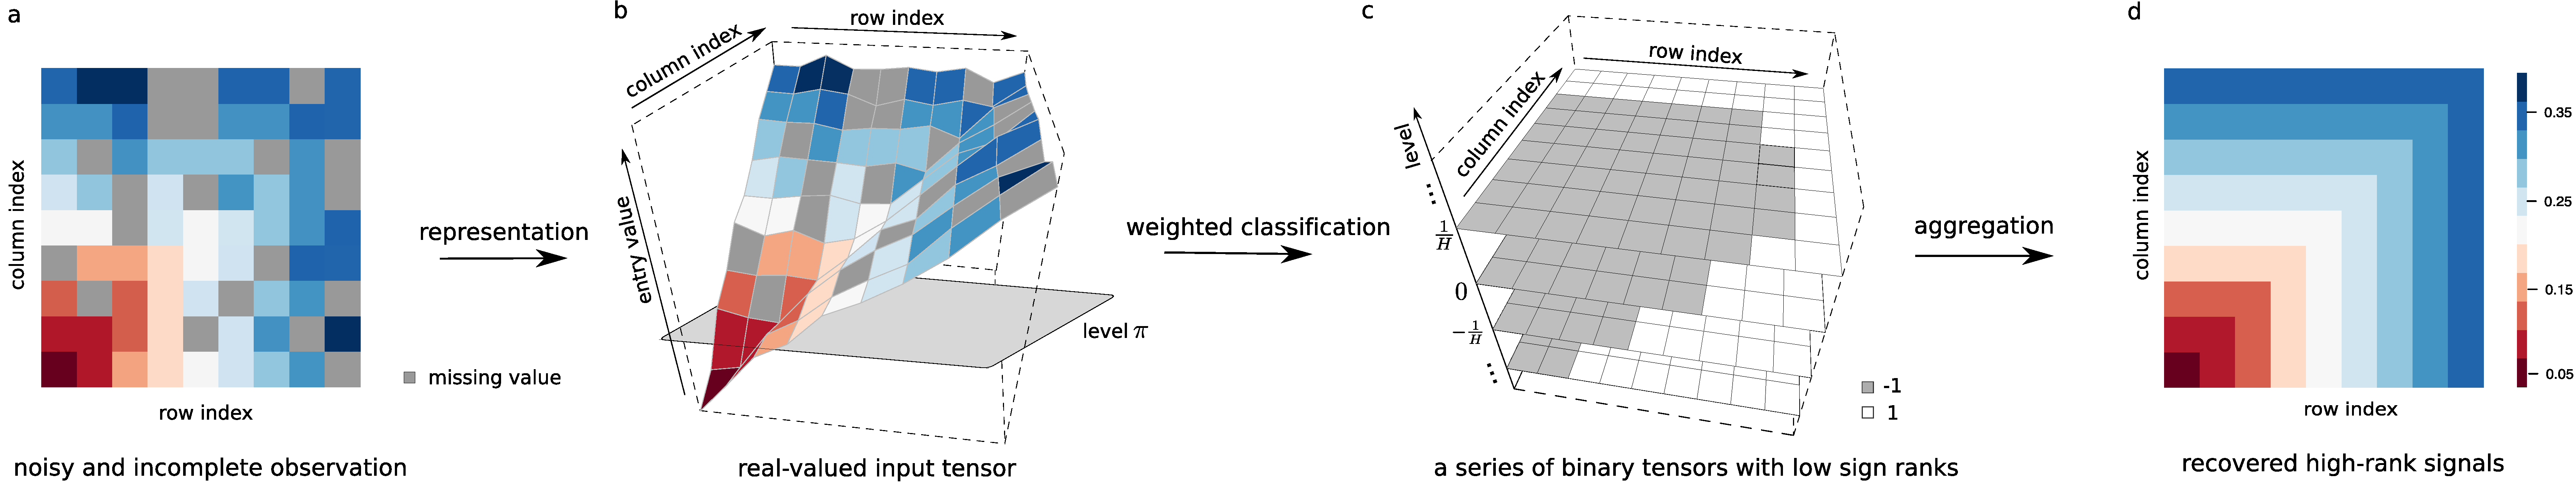
\includegraphics[width=1\textwidth]{image_new2.pdf}}
\caption{Illustration of our proposed method. For visualization purpose, we plot an order-2 tensor (a.k.a. matrix) in the figure; similar procedure applies to higher-order tensors. (a): input tensor $\tY_\Omega$ with noisy and incomplete entries. (b) and (c): the algorithm uses weighted classification to estimate sign tensors $\sign(\Theta-\pi)$ for a sequence of levels $\pi\in \{-1,\ldots,-{1\over H},0,{1\over H},\ldots,1\}$. (d) output tensor $\hat \Theta$ with denoised and imputed entries. The depicted example is based on Example 5, where the true signal matrix has full rank. }\label{fig:demo}
\end{figure*}

Our observation is an incomplete data tensor from~\eqref{eq:model}, denoted $\tY_\Omega$, where $\Omega\subset[d_1]\times\cdots\times[d_K]$ denotes the index set of observed entries. We consider an observation model of $\Omega$ that allows both uniform and non-uniform sampling. Specifically, let $\Pi=\{\pi_\omega\}$ be an arbitrarily predefined probability distribution over the full index set such that $\sum_{\omega\in[d_1\times \cdots \times d_K]}\pi_\omega=1$. We assume the entries $\omega$ in $\Omega$ are i.i.d.\ draws with replacement from the full index set using distribution $\Pi$. The sampling rule will be denoted as $\omega\sim \Pi$.

Our goal is to accurately estimate $\Theta$ from the incomplete, noisy observation $\tY_\Omega$. In particular, we focus on the following two problems:
\begin{itemize}[leftmargin=*]
\item Q1 [Nonparametric tensor estimation]. How to flexibly estimate $\Theta$ under a wide range of structures, including both low-rankness and high-rankness?
\item Q2 [Tensor Completion]. How many observed tensor entries do we need to consistently estimate the signal $\Theta$?
\end{itemize}


\subsection{Inadequacies of common low-rank models}
The signal plus noise model~\eqref{eq:model} is common in tensor literature. Most existing methods perform estimation based on the low-rankness of $\Theta$~\cite{anandkumar2014tensor,montanari2018spectral,kadmon2018statistical,cai2019nonconvex}. While these methods have shown great success in low-rank recovery, little is explored when the underlying signal tensor is of high rank. Here we provide two examples to illustrate the limitation of classical low-rank models.

The first example reveals the sensitivity of tensor rank to order-preserving transformations. Let $\tZ \in \mathbb{R}^{d\times d\times d}$ be an order-3 tensor with $\text{rank}(\tZ)=3$. Suppose a monotonic transformation $f(z)=(1+\exp(-cz))^{-1}$ is applied to $\tZ$ entrywise, and we observe data from model~\eqref{eq:model} with the signal tensor $\Theta=f(\tZ)$. Figure~\ref{fig:example}a plots the numerical rank of $\Theta$ versus $c$ when the tensor dimension $d=30$. As we can see, the rank increases rapidly with $c$, rending traditional low-rank tensor methods ineffective in the presence of order-preserving nonlinearities. In applications such as digital processing and genomics analysis, the tensor of interest often undergoes some unknown transformation prior to measurements. The sensitivity to transformation therefore makes the low-rank model less desirable in practice. 

The second example shows that the classical low-rankness may exclude interesting tensor structures. Here we consider the signal tensor of the form $\Theta=\log(1+\tZ)$, where $\tZ$ is an order-3 tensor with entries $\tZ(i,j,k)={1\over d}\max(i,j,k)$ for $(i,j,k)\in[d]^3$. In this example neither $\Theta$ nor $\tZ$ is low rank; in fact, we are able to show that both tensor ranks are lower bounded by dimension $d$ (see proofs in Appendix and Figure~1b). The matrix analogy of this structured $\Theta$ was first studied in~\citet{chan2014consistent} in the context of graphon analysis. However, classical tensor models fail to incoporate these types of structures.  

\begin{figure}
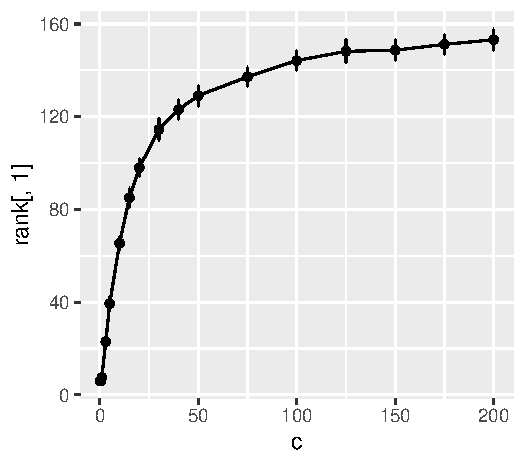
\includegraphics[width=3.9cm]{example1.pdf}
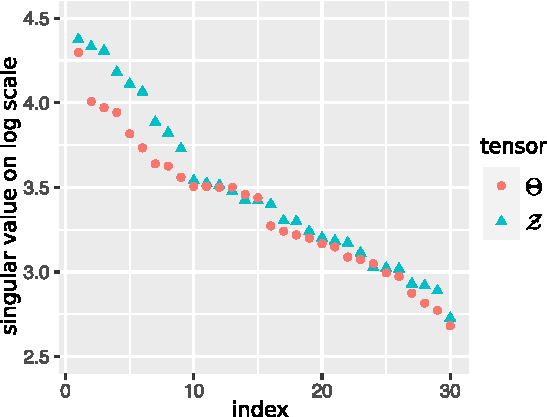
\includegraphics[width=4.2cm]{example2.pdf}
\caption{(a) Numerical rank of $\Theta=f(\tZ)$ versus $c$ in Example 1. Here $\tZ$ is generated using a rank-3 tensor whose (unnormalized) eigenvectors consist of i.i.d.\ entries from $N(0,1)$. The numerical rank is computed as the minimal $R$ such that $\min_{\rank(\tA)\leq R}{ \FnormSize{}{\Theta-\tA}\over \FnormSize{}{\Theta}} \leq 0.1$. (b). Top $d=30$ numerical singular values of tensors $\Theta$ and $\tZ$ in Example 2. The reported values in both figures are obtained by running CP decomposition ten times using random initializations. }\label{fig:example}
\end{figure}
In the above and many other examples, the signal tensor of interest is structured but of high rank. %We argue that, this low-rankness is restricted, and not necessarily for accurate recovery. 


%\begin{example}[Binary tensor]
%For a binary tensor $\tY\in\{0,1\}^{d_1\times \cdots \times d_K}$, the entries in the noise $\tE=\tY-\mathbb{E}(\tY)$ are bounded by $1/4$. 
%\end{example}

%\subsection{Algebraic properties of low sign rank tensors}
\subsection{Overview of our proposal}
Before describing the main results, we outline the main crux of our idea. In the earlier two examples, the tensor $\Theta$ is of high rank. However, the runcated $(\Theta-\pi)$ has the same sign pattern as low-rank tensors. This observation suggests a  a more general framework that allows flexibly modeling..... Indeed as we see in Section~\ref{sec:method}, the model not only corporates common low-rank models such as CP/Tucker and single index model, but also allows substantial class of structured tensors. 

Figure~\ref{fig:demo} illustrates the main approach of our method. We convert the data tensor into a tensor series $\bar \tY_\pi= (\tY-\pi)$ for $\pi\in \tH=\{-1,\ldots, {\scriptstyle -{1\over H}},0,{\scriptstyle {1\over H}},\ldots,1\}$ and perform classification to estimate the sign signal of each, 
\[
\hat \tZ_\pi=\argmin_{\text{$\tZ\in $ classifier model}} \risk(\tZ,\ \sign \bar \tY_\pi).
\]
Then, the nonparametric estimate takes the form of
\[
\hat \Theta = {1\over 2H+1}\sum_{\pi \in \tH} \sign(\hat \tZ_\pi).
\]
Here $\risk_\pi(\cdot,\cdot)$ is a weighted extension of usual classification risk, and the classifier models refer to a tensor model which will be described in next section. 

The main approach is to estimate $\hat \Theta$ from the binary tensor series $\{\sign(\tY-\pi)\colon \pi \in \tH\}$. 1) exactly recover the signal tensor under a wide range of currently used tensor models; 2) brings the benefit of high-rank tensor estimation and completion; 3) leverage efficient classification algorithms. 
We choose the classifier model that is broader that incorporates low rank tensor model, single index tensor model, and nonlinear tensor model, etc, in the literature. It may be counterintuitive that dichotomization may lose information in the data. It turns out the ensemble model based on dichotomizations not only preserves all information in the data, but also brings the nonparametric benefit of model-free and flexibility over classical parameter models.


\section{Sign representable tensors}
In this section, we introduce the sign representable tensors and the properties of sign tensor series. 

\subsection{Sign rank of tensors}
Let $\Theta$ be a real-valued tensor, and $\sign (\Theta)$ be the induced sign tensor.  
The sign pattern induces an equivalence relationship between tensors. Two tensors are called sign equivalent, denoted $\simeq$, if they share the same sign pattern. 

\begin{defn}[Sign rank]
%We call a tensor has a low sign rank, if for every $\pi \in [-L, L]$, $\sign (\Theta - \pi ) = \sign (\tM)$, where $\tM$ is a tensor with Tucker rank bounded by $\mr$.
The sign rank of a tensor $\Theta$ is the minimal rank among all tensors that share the same sign pattern as $\Theta$,
\[
\srank(\Theta) = \min \{\rank(\Theta')\colon  \Theta'\simeq \Theta,\ \Theta'\in\mathbb{R}^{d_1\times \cdots \times d_K}\}.
\]
\end{defn}
The sign rank is also called \emph{support rank}~\cite{cohn2013fast}, \emph{minimal rank}, \emph{nondeterministic rank}~\cite{de2003nondeterministic}, in the filed of combinatorics and computational complexity. Some literature defines sign rank for binary tensors/matrices only; we extend the notion to real-valued tensors. Note that the sign rank concerns only the sign pattern of $\Theta$ but discards the magnitudes information. In particular, $\srank(\Theta)=\srank(\sign \Theta)$. 
%\begin{proof} 
%Consider a tensor $\Theta=\entry{\Theta_{ijk}}\in\{-1,1\}^{d\times d\times d}$ with entries $\Theta(i,j,k)=-1$ if $i=j$ and $\Theta(i,j,k)=1$ otherwise. Then the tensor has usual rank $d$, but its srank equals to 2. 
%$\rank(\Theta)=\rank(\Theta(\cdot,\cdot,1))=d, \srank(\Theta)=\srank(\Theta(\cdot,\cdot,1))=2$.
%\end{proof}
%We use $\caliP(r)=\{\Theta \colon\srank(\Theta)\leq r, \maxnormSize{}{\Theta}\leq 1\}$ to denote the family of tensors with sign rank bounded by $r$. The sign pattern induces an equivalent class in the tensor family. Two tensors are called equivalent if they share the same sign pattern. We will use $\sign (\Theta)$ to denote the equivalent that share the $\{\tS\colon \sign (\tS)=\sign (\Theta)\}$. Note that $\tS$ itself may be even full rank, although it shares the same sign pattern as a low rank tensor $\sign (\Theta)$. 

Determining the sign rank is NP hard, just as the determining tensor rank is NP hard. Fortunately, many tensors arising in practice have low sign rank. We show here the family of low rank sign tensors is strictly larger than usual low rank tensors. By definition, the sign rank is upper bounded by the usual rank. More generally, 
\begin{cor}[Upper bounds of sign rank]~\label{cor:monotonic} For any monotonic function $g\colon \mathbb{R}\to \mathbb{R}$ with $g(0)=0$, 
\[
\textup{srank}(\Theta)\leq\rank(g(\Theta)).
\]
\end{cor}
Conversely, we show that the sign rank can be dramatically smaller than tensor rank. 
\begin{prop}[Strictness]\label{prop:extention}For every order $K$ and tensor dimension $d$, there exists a tensor whose usual rank is $d$ but the sign rank is 2. 
\end{prop}
The Proposition~\ref{prop:extention} is shown by construction, and we provide the proof in Appendix. Corollary~\ref{cor:monotonic} and Proposition~\ref{prop:extention} demonstrates that low sign rank tensors constitute a strictly broader family than the usual low rank tensors. Some examples include identity tensors, banded tensor, ... etc. ...


We now introduce the family of tensor model~\eqref{eq:model} of our interest, which we coin as ``sign representable tensors''.
%Note that $\caliP$ concerns only the sign, but not the magnitude, information of entries in $\Theta$. 
%and $\caliP(r)=\cap_{\pi\in[-1,1]} \caliP(r,\pi)$
\begin{defn}[Sign representable tensors] 
Fix a level $\pi\in[-1,1]$. A tensor $\Theta$ is called $(r,\pi)$-sign representable, if the tensor $(\Theta-\pi)$ has sign rank bounded by $r$. %The tensor model~\eqref{eq:model} is called locally low sign rank at $\pi$ if the affine tensor $(\Theta-\pi)$ has low sign rank, i.e.,
%\[
%\Theta-\pi \in \caliP(r).
%\]
The binary tensor $\sign(\Theta-\pi)$ is called the $\pi$-level sign tensor.
If a tensor $\Theta$ is $(r,\pi)$-sign representable for all $\pi\in[-1,1]$ except for a finite number of points, then we say that $\Theta$  is $r$-globally sign representable, denoted $\Theta \in \caliP(r)=\{\Theta\colon \srank(\Theta-\pi)\leq r \text{ for all }\pi\in[-1,1]\}$.
\end{defn}
%\begin{assumption}[Structural assumption] Assume $\Theta$ in model~\ref{eq:model} belongs to $\caliP(r)$.  
%\end{assumption}

 We show that the $r$-globally sign representable tensor is very broad family that incorporates many usual common tensor models, such as single index model, GLM models, and certain hypergraphon models. 

{\color{red}emphasize the original tensor may be high rank....Give a toy example.}

\begin{example}[CP/Tucker low-rank tensor model] Let $\Theta$ be a tensor with CP rank bounded by $r$. Then the usual signal + noise model is a special cases of low sign rank tensor assemble model. 
\end{example} 

\begin{example}[Generalized linear model (GLM) for tensors] Let $\tY$ be a binary tensor. Then the GLM low rank model is a special case of low sign rank tensor assemble model. 
\end{example}

\begin{example}[Single index model]
Suppose there exists a (unknown) monotonic function $g\colon \mathbb{R}\to \mathbb{R}$ such that $g(\Theta)$ has rank bounded by $r$. Then, $\Theta$ belongs to the a low sign rank assemble tensor; i.e.,  $\Theta\in \caliP(r+1)$.
\end{example}

\begin{example}[Tensor block model]
Finite possible $\pi$. Suppose $\Theta$ has at most $r$ multiway blocks. Then $\Theta \in \caliP(r)$. 
\end{example}

\begin{example}[Min/Max hypergraphon]
Suppose the matrix $\Theta=\entry{\Theta(i,j,k)}$ are generated from the graphon model,
\[
\Theta(i,j,k)=\exp(1+0.5\max(x_i,y_j,z_k)), 
\]
where $x_i, y_i,z_k \sim \text{Uniform}[0,1]$ i.i.d.\ for all $(i,j,k)\in[d_1]\times[d_2]\times[d_3]$. Then the affine matrix $(\Theta-\pi)$ has sign rank bounded by 2; i.e., $\Theta \in \caliP(2)$ for every tensor dimension. In contrast, the regular matrix rank of $\Theta$ has full rank almost surely for every matrix dimension $d$. This example highlights the benefit of our assemble model. 

%More generally, for functions $\Theta_{ijk}=g(x_i,y_j,z_k)$ that is monotonic in each variable, the affine matrix $(\Theta-\pi)$ has low sign rank. Equivalently, there exists permission such that $\Theta_{ijk}\geq \max(\Theta_{ij'k'},\Theta_{i'jk'},\Theta_{i'j'k})$ for all $i',j',k'$. 
More generally, if $\Theta(i,j,k)=g(\max(x_i,y_i,z_i))$ where $g(\cdot)$ is a continuous function with at most $r$ real roots in the equation $g(z)=\pi$ (for example, this holds for all $\pi\in[-1,1]$ when $g$ is an $r$th polynomial.) Then $\Theta \in \caliP(r+1)$. Same properties hold if the maximum is replaced by minimum. 
\end{example}

%\begin{prop} Suppose $\Theta$ is tensor with $\mnormSize{}{\Theta}\leq1$, and $\Pi$ is a sequence of $(2H+1)$ evenly spaced points in $[-1,1]$. Then
%\[
%\textup{Loss}(\Theta,\ {1\over 2H+1}\sum_{\pi \in\Pi} \sign(\Theta-\pi)) \leq {1\over H}.
%\]
%\end{prop}

\subsection{Characterization of sign tensors via weighted classification}

Accurate estimation of sign representable tensors crucially depends on the behavior of sign tensors, $\sign(\Theta-\pi)$. In this section, we show that weighted classification completely characterizes the sign tensors. The results bridge the algebraic and statistical properties of sign representable tensors, and provide a building block for our nonparametric algorithm (see Figure~\ref{fig:demo}).
 
 For a given $\pi \in [-1,1]$, define a new data tensor $\bar \tY = (\tY-\pi)$. We introduce a weighted classification loss function
\[
L(\tZ, \bar \tY)= \sum_{\omega \in \Omega}\KeepStyleUnderBrace{|\bar \tY(\omega)|}_{\text{entry-specific weight}} \times \KeepStyleUnderBrace{| \sign \tZ(\omega)-\sign \bar \tY(\omega|)}_{\text{classification loss}},
\]
where $\tZ\in\mathbb{R}^{d_1\times \cdots \times d_K}$ is the decision variable to be estimated. In the case of binary tensor, taking $\pi=1/2$ gives unweighted usual classification risk.


Denote the weighted classification risk 
\begin{equation}\label{eq:population}
\textup{Risk}(\tZ)=\mathbb{E}_{\tY,\Omega}L(\tZ,\bar\tY),
\end{equation}
where the expectation is taken with respect to both $\tY$ under the sign assemble model, and $\Omega$ under the sampling distribution. The form of $\textup{Risk}(\cdot)$ implicitly depends on $\pi$. 
\begin{prop}[Global optimum of weighted risk] Suppose the data $\tY$ is generated from model~\ref{eq:model} with $\Theta \in \caliP(r)$. Then, for all $\bar \Theta$ that are sign equivalent to $\sign(\Theta-\pi)$, 
\begin{align}
\textup{Risk}(\bar \Theta )&=\min\{\textup{Risk}(\tZ)\colon \tZ\in\mathbb{R}^{d_1\times \cdots \times d_K}\},\\
&=\min\{\textup{Risk}(\tZ)\colon \textup{rank} \tZ\leq r\}.
\end{align}
\end{prop}
The support sign tensor $\sign(\Theta-\pi)$ serves the bridge between the target parameter $\Theta$ and statistical properties of $\textup{Risk}(\cdot)$. 
{\color{red} Highlight the importance of weight!}

The above property shows that the $\sign(\Theta-\pi)$ is one of the optimum of $\risk(\cdot)$. However, the converse may not true. We establish the uniqueness; that is, is the tensor $\sign(\Theta-\pi)$ the unique (up to sign equivalence) optimizer of $\risk(\cdot)$? The following assumption quantifies the identifiability of $\bar \Theta$ from $\risk(\cdot)$. 


%Suppose the entries in the index set $\Omega$ are i.i.d.\ sampled with replacement from the entire index set using a probability $\Pi$ over $[d_1]\times\cdots\times[d_K]$. We use $\omega\sim \Pi$ for $\omega\in[d_1]\times\cdots\times[d_K]$ to denote this observation model. 
%The underlying tensor $\Theta$ and the sampling distribution $\omega\sim \Pi$ induces a [-1,1]-valued random variable $\Theta(\omega)$. We use $\mathbb{P}_{\omega\sim \Pi}$ to denote the distribution law over for $\Theta(\omega)$. 
%\begin{enumerate}
%\item $(\omega)\sim\Pi$
%\item Marginal distribution $\Theta(\omega) & \sim \tF, \ \text{for each }\omega\in[d_1]\times\cdots\times[d_K]$,\\
%\item Jointly $\srank(\Theta-\pi)& \leq r, \ \text{for }\pi\in[0,1]$
%\end{enumerate}

We introduce some additional notation. Recall that $\omega\in \Pi$ denotes the sampling distribution over index set. Our theory concerns the high-dimensional ... Both $\Pi$ and $\Theta$ implicitly depend on the tensor dimension. We are interested in the high dimensional region $d:=\min_kd_k\to\infty$ for the sequence $\Pi=\Pi_d$ and $\Theta=\Theta_d$. Unless otherwise stated, all relevant assumptions should be interpreted as uniform conditions that hold for all $d$. 
%Let $\hat F(t)={1\over d^K}\sum_{\omega\in[d]^K}\mathds{1}(\Theta_d(\omega)\leq t)$ be the marginal empirical cumulative distribution function (CDF) of signal entries. Assume $\hat F(t)\to F(t)$ for every value of $t$ as $d\to\infty$. 
Let $\tN=\{\pi\colon \mathbb{P}_{\omega\sim \Pi}(\Theta(\omega)=\pi)\neq 0\}$ denote the set of mass points of $\Theta(\omega)$. Assume there exists a constant $c_1>0$, independent of tensor dimension, such that $|\tN|\leq c_1$. Furthermore, 

\begin{assumption}[$\alpha$-smoothness]\label{ass:margin} 
Fix $\pi\notin \tN$. Assume there exist constants $\alpha=\alpha(\pi), c=c(\pi) >0$, independent of tensor dimension, such that, 
\begin{equation}\label{eq:smooth}
\sup_{0\leq t<\rho(\pi, \tN)}{\mathbb{P}_{\omega \sim \Pi}(\omega \colon |\Theta (\omega)-\pi|\leq t )\over t^\alpha} \leq c,
\end{equation}
where $\rho(\pi,\tN):=\min_{\pi'\in \tN}|\pi-\pi'|$ denotes the distance from $\pi$ to the nearest point in $\tN$. The largest possible $\alpha=\alpha(\pi)$ is called the smoothness index at level $\pi$. We make the convention that $\alpha= \infty$ if the set $\{\omega\colon |\Theta(\omega)-\pi|\leq t\}$ is measure-zero set, implying the density of $\Theta(\omega)$ has a jump around the level $\pi$.
\end{assumption}

If $\Theta$ is $\alpha$-smooth for all $\pi\in[-1,1]$ except for a finite number of points, then we call $\Theta$ is $\alpha$-globally smooth. 
The smoothness index is determined by the marginal density of $\Theta(\omega)$, or equivalently, by the underlying $\Theta$ and the sampling distribution $\omega\sim \Pi$. 

To gain some intuition about~\eqref{eq:smooth}, we consider the case of uniform sampling model where each tensor entry has equal probability to be observed. Larger value of $\alpha$ corresponds to an easier problem (faster statistical rate). The case $\alpha<1$ may indicate a local extremum or inflection point of the density of $\Theta(\omega)$ at the level $\pi$. Typical cases are $\alpha=1$, for example, when the density of $\Theta(\omega)$ is locally bilipschitz. 

For tensor block models, $|\tN|$ equals the number of blocks with distinct means which is finite. Furthermore, we can take $\alpha= \infty$ for all $\pi \notin \tN$ (because the numerator in~\eqref{eq:smooth} is zero). For max/min hypergraphon model with $r$-th polynomial function, we have $\alpha=1$ for all $\pi$ except at most $r$ many points (local extremums). For single index model $f(\Theta)$....

We consider the mean absolute error (MAE)
\[
\text{MAE}(\Theta_1, \Theta_2)\stackrel{\text{def}}{=}\mathbb{E}_{\omega\sim \Pi}\onenormSize{}{\Theta_1-\Theta_2}.
\]

We now reach the main theorem in this section. 
\begin{thm}[Identifiability] Under Assumption~\ref{ass:margin}, for tensors $\bar \Theta \simeq \sign(\Theta-\pi)$ and all tensors $\tZ\in\mathbb{R}^{d_1\times \cdots \times d_K}$,
\[
\textup{MAE}(\sign \tZ, \sign \bar \Theta) \leq C(\pi)\left[\textup{Risk}(\tZ)-\textup{Risk}( \bar \Theta)\right]^{\alpha/(1+\alpha)},
\]
where $C(\pi)>0$ is a constant. 
\end{thm}
The result immediately suggests uniqueness of the optimizer of $\text{Risk}(\cdot)$ up to a zero-measure set under $\Pi$. Furthermore, it establish the stability of recovering $\sign \Theta$ from the optimization~\eqref{eq:population}.  
%Second, the empirical optimizers is still non-unique, because any tensor $\hat \tZ'$ that share the same sign pattern as $\hat \tZ$ are the solution. To make the optimization well posed, we propose the following minimal-norm optimization
\section{Nonparametric tensor completion via sign series}

Now, we are ready to state the assemble algorithm. We use the sample formulation ... , and propose the estimate
\begin{equation}\label{eq:estimate}
\hat \tZ_\pi = \argmin_{\tZ\colon \text{rank}(\tZ)\leq r, \ \FnormSize{}{\tZ}\leq 1} L(\tZ,\bar \tY_\pi),
\end{equation}
for a series of levels $\pi \in \tH=\{-1,\ldots,-{1\over H}, 0, {1\over H},\ldots,1\}$, and the aggregated tensor estimate
\[
\hat \Theta = {1\over 2H+1}\sum_{\pi \in \tH}\sign{\hat \tZ_\pi}.
\]
%In order to establish the accuracy of $\hat Z$ to $\bar \Theta$. 
%\begin{equation}\label{eq:estimate}
%\hat \tZ_\lambda = \argmin_{\tZ\in \caliP(r)} L(\tZ, \tY).
%\end{equation}
%Here $\lambda$ is a tuning parameter; when $\lambda \to 0$, the solution converges to the minimal-norm optimizer. %Let $\Pi=\{\pi_\omega\}$ denote the sampling distribution over the index set $d_1\times \cdots \times d_K$ such that $\sum_{\omega}\pi_\omega=1$. 
%We define the weighted classification error (CErr) between two binary tensors $\tA, \tB \in \{-1,1\}^{d_1\times \cdots \times d_K}$.
%\[
%\text{CErr}(\tA,\tB)=\mathbb{E}_{\Omega \sim \Pi}\onenormSize{}{\tA-\tB}=\sum_{\omega}\pi_\omega|\tA(\omega)-\tB(\omega)|.
%\]

%\begin{assumption}\label{ass} Fix a $\pi\in[-L,L]$. Assume there exist constants $\delta=\delta(\pi)>0$ and $C=C(\pi)>0$, independent of tensor dimension, such that
%\[
%\mathbb{P}_{\Omega\sim \Pi}(\omega \colon |\bar \Theta (\omega)|\leq t ) \leq Ct^\alpha, \ \text{for all }t\in(0,\delta).
%\]
%\end{assumption}
\begin{thm}[Estimation of sign series]\label{thm:classification} Suppose $\Theta\in\caliP(r)$ and Assumption~\ref{ass:margin} holds at level $\pi\notin \tN$ with smoothness index $\alpha\in[0,1]$. Then, for every such $\pi$, with very high probability over $\tY_\Omega$, 
\[
\textup{MAE}(\sign \hat \tZ_\pi, \sign \bar \Theta_\pi) \lesssim \left({d r \over |\Omega|}\right)^{\alpha/(\alpha+2)}+{1\over \rho^2(\pi, \tN)} {dr \over |\Omega|}.
\]
\end{thm}
Theorem~\ref{thm:classification} shows that the estimate from~\eqref{eq:estimate} recovers the desired sign tensor $\sign \bar \Theta$. 
%\begin{cor}[Excess risk and generalization error]
%\[
%\risk(\hat \tZ_\pi)-\risk(\bar \Theta) \leq C(\pi)\left({d r \over |\Omega|}\right)^{(\alpha+1)/(\alpha+2)}.
%\]
%\end{cor}
%Compared to generalization risk, with probability $1-\delta$
%\[
%|\risk(\hat \tZ)-L(\hat \tZ, \tY)| \leq \sqrt{dr\over |\Omega|}+{\delta \over |\Omega|}.
%\]
The result suggests the sample complexity for sign tensor recovery is of the order $dr$. We will show that later, this complexity remains for recovering the entire tensor. 
%we consider the mean absolute error (MAE)
%\[
%\text{MAE}(\Theta_1, \Theta_2)\stackrel{\text{def}}{=}\mathbb{E}_{\omega\sim \Pi}\onenormSize{}{\Theta_1-\Theta_2}.
%\]
\begin{thm}[Tensor estimation error] With very high probability over $\tY_\Omega$,
\[
\textup{MAE}(\hat \Theta, \Theta)\leq \left({d r \over |\Omega|}\right)^{\alpha/(\alpha+2)}+{1\over H}+H{d r \over |\Omega|}.
\]
Setting $H\asymp \left( |\Omega|\over rd\right)^{1/2}$ gives
\[
\textup{MAE}(\hat \Theta, \Theta)\leq \left(dr \over|\Omega|\right)^{{\alpha \over \alpha+2} \vee {1\over 2}}.
\]
\end{thm}

\begin{cor}[Sample complexity for completion] With very high probability 
\[
\textup{MAE}(\hat \Theta, \Theta)\to 0, \quad \text{as}\quad {|\Omega|\over d_{\max}}\to \infty.
\]
\end{cor}

Completion is consistent provided that $|\Omega|/dr\to\infty$. Furthermore, in the full observation case, $|\Omega|=\prod_k d_k$, then the 
\[
\textup{MAE}(\hat \Theta, \Theta)\leq \left(r\over d^{-(K-1)}\right)^{{\alpha \over \alpha+2} \vee {1\over 2}}.
\]
%For tensor block model $\alpha=\infty$, we have ${1\over 2}$. For single index model ${1\over 3}$. 

\begin{example}[Tensor block model]
Consider tensor block model. $\alpha=\infty$. Earlier results show the estimation error
\[
\textup{MAE}(\hat \Theta, \Theta)\leq \sqrt{r\log d \over |\Omega|}.
\]
this is the best rate. reached the minimax rate??
\end{example}
\begin{example}[Single index tensor model]
$\tO(1/3)$???
\end{example}
%\begin{thm}[Minimax rate] Because our function class incorporates the tensor block model, the following results immediately follows from the minimax rate for tensor block model
%\[
%\inf_{\hat \Theta}\sup_{\Theta \in \caliP(r)} {1\over n^2}\mathbb{E}\FnormSize{}{\hat \Theta - \Theta} \geq {rd\over |\Omega|},
%\]
%when $\alpha=1$. 
%\end{thm}

\section{Algorithm}
The optimization~\eqref{eq:estimate} is a non-convex problem because of the nonconvexity in $L$ and the rank constraints. We present an efficient ADMM algorithm with a good empirical performance. 

\begin{align}
\min_{\tZ}L(\tZ)&:={1\over |\Omega|}\sum_{\omega \in \Omega}|\bar y_\omega| (1-z_\omega\bar y_\omega)_{+}\\
\text{subject to }&\rank(\tZ)\leq r \ \text{and }\FnormSize{}{\tZ}\leq 1.
\end{align}

\begin{align}
L(\tZ,\tW,\Lambda,\rho,\lambda)&={1\over |\Omega|}\sum_{\omega \in \Omega}|\bar y_\omega| (1-z_\omega\bar y_\omega)_{+}\\
&+\lambda\FnormSize{}{\tZ}^2+
\rho \FnormSize{}{\tZ-\tW}^2 + \langle \tZ-\tW,\Lambda \rangle
\end{align}
Two changes: 1. make convex relaxation; 2. alternatively... Gradually increasing $\rho$ and $\lambda$.


\clearpage
\begingroup
\let\clearpage\relax 
\onecolumn 
\begin{proof}
We verify two conditions. 
\begin{enumerate}
\item Approximation error. For $\tZ$ with $\text{rank}(\tZ)\leq r$, we have $\textup{Risk}(\tZ)-\textup{Risk}(\bar \Theta)=0$ for all $d$.  
\item Variance-to-mean relationship
\[
\text{Var}_{\tY, \Omega}[L(\tZ,\bar \tY_\pi)-L(\bar \Theta, \tY_\pi)]\leq [\textup{Risk}(\tZ)-\textup{Risk}(\bar \Theta)]^{\alpha/(1+\alpha)}+{1\over \rho(\pi, \tN)}[\textup{Risk}(\tZ)-\textup{Risk}(\bar \Theta)].
\]
Apply Lemma~\ref{lem:tensor} to the above condition, we obtain
\[
\textup{Risk}(\tZ)-\textup{Risk}(\bar \Theta)\leq t_n^{(\alpha+1)/(\alpha+2)}+{1\over \rho(\pi, \tN)}t_n, \quad \text{where }t_n={Krd\over n}.
\]
\end{enumerate}
\end{proof}

\begin{lem}\label{lem:tensor}

Because the classification rate is scale-free; $\text{Risk}(\tZ)=\text{Risk}(c\tZ)$ for every $c>0$. Therefore, without loss of generality, we solve the estimate subject to $\FnormSize{}{\tZ}\leq 1$,
\[
\hat \tZ=\argmin_{\tZ\colon \textup{rank}(\tZ)\leq r, \FnormSize{}{\tZ}\leq 1}L(\tZ,\bar \tY_\pi).
\]
Write $|\Omega|=n$. We have
\[
\mathbb{P}[\textup{Risk}(\hat \tZ)-\textup{Risk}(\bar \Theta)\geq t_n]\leq {7\over 2}\exp(-Cnt_n).
\]
The rate of convergence $t_n>0$ is determined by the solution to the following inequality,
\[
{1\over t_n}\int^{\sqrt{t_n^\alpha+\rho^{-1}t_n}}_{t_n} \sqrt{\tH_{[\ ]}(\varepsilon,\ \tF,\ \vnormSize{}{\cdot}) }d\varepsilon \leq n^{1/2}, 
\]
where $\tF=\{\tZ\colon \textup{rank}(\tZ)\leq r, \ \FnormSize{}{\tZ}^2\leq 1\}$ and $\rho=\rho(\pi, \tN)$. By Lemma~\ref{lem:bracketing}, we obtain 
\[
t_n\asymp \left({Kdr\over n}\right)^{(\alpha+1)/(\alpha+2)} +{1\over \rho^2(\pi, \tN)} {Kdr\over n}.
\] 
Finally, we obtain
\[
\mathbb{P}[\textup{Risk}(\hat \tZ)-\textup{Risk}(\bar \Theta)\geq t_n]\leq {7\over 2}\exp(-Cd^{\alpha+1\over \alpha+2}n^{1\over \alpha+2}) \leq {7\over 2}\exp(-C\sqrt{d}),
\]
where $C=C(k,r)>0$ is a constant independent of $d$ and $n$.  
\end{lem}

\begin{lem}[Bracketing number for bounded low rank tensor]\label{lem:bracketing}
\[
\sqrt{\mathbb{E}_{\omega\sim \Pi}|\tZ_1(\omega)-\tZ_2(\omega)|^2} \leq \mnormSize{}{\tZ_1-\tZ_2} \leq \FnormSize{}{\tZ_1-\tZ_2}.
\]
Therefore
\[
\tH_{[\ ]}(2\varepsilon, \tF, \vnormSize{}{\cdot})\leq \tH(\varepsilon, \tF, \FnormSize{}{\cdot}) \leq C{(1+Kdr)\log {d\over \varepsilon}},
\]
where the covering number for low rank tensor is based on~\citep{mu2014square,9119759}.
\end{lem}

\endgroup


\bibliographystyle{chicago}

\bibliography{tensor_wang}

\appendix

\end{document}
